%% ----------------------------------------------------------------
%% Article.tex
%% ---------------------------------------------------------------- 
\documentclass{ecsarticle}     % Use the Article Style
\graphicspath{{Figures/}}   % Location of your graphics files
\usepackage{natbib}            % Use Natbib style for the refs.
\hypersetup{colorlinks=false}   % Set to false for black/white printing
\input{Definitions}            % Include your abbreviations

\usepackage[nodayofweek]{datetime}
\usepackage{listings}
\usepackage{color}

\usepackage{graphicx}



%% ----------------------------------------------------------------
\begin{document}
\frontmatter
\title      {COMP6036: Advanced Machine Learning\\[1cm]
            An investigation into DBSCAN}
      
\addresses  {\deptname\\\univname}
\authors                 {\href{mailto:ajr2g10@ecs.soton.ac.uk}{Ashley J. Robinson}\\\href{mailto:ajr2g10@ecs.soton.ac.uk}{ajr2g10@ecs.soton.ac.uk}}

\date       {\today}
\subject    {}
\keywords   {}
\maketitle
%% ----------------------------------------------------------------



\begin{abstract}
Your abstract goes here
\end{abstract}

\mainmatter


\section{Motivation for Algorithm}

DBSCAN (Density-Based Spatial Clustering of Applications with Noise) is an application of machine learning introduced by~\cite{ester96dbscan}.
Intended to address Spatial Database Systems (SDBS) which can be produced from natural geometric and geographical datasets or applications such a layout for integrated circuit design~\citep{guting94sdbs}.
It has three main objectives.
To minimise the required domain knowledge needed to set input parameters, have the capability to discover clusters of arbitrary shapes and to perform well on large spatial databases.

At the time of creation the algorithms was compared to a recent development called CALARANS~\citep{ng94clarans} which is an extension of CLARA (Clustering LARge Applications)~\citep{kaufman90clara}.
Both algorithms are intended for use on large databases but CLARANS uses random noise to improve performance.
Apart from traditional clustering algorithms, such a K-means, DBSCAN was a breakthrough in terms of a density approach to datasets.

\section{Technical Explanation}

DBSCAN uses cluster density to classify data.
It tries to find connectivity between data poiunts within a reasonable distance.
This distance is passed to algorithm as an input parameter and can be tuned to give

The graphs in Figure~\ref{fig:compare} are different clustering algorithms applied to a shape dataset taken from~\cite{gionis05cluster}. 
Algorithms were taken from a machine learning toolbox for Python~\citep{scikit13ml}. 
\begin{figure}[ht]
   \centering
   \subfigure[K-Means]{
      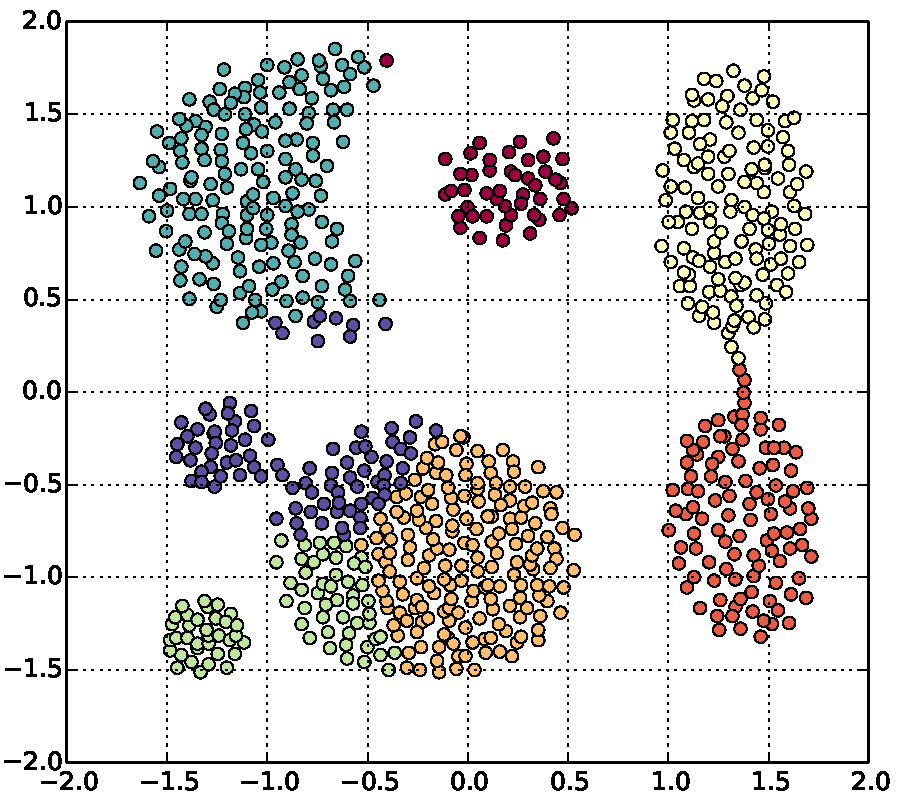
\includegraphics[height = 5cm,width = 5cm]{kmeans.pdf}
      \label{fig:kmeans}
   }
   \subfigure[WARD]{
      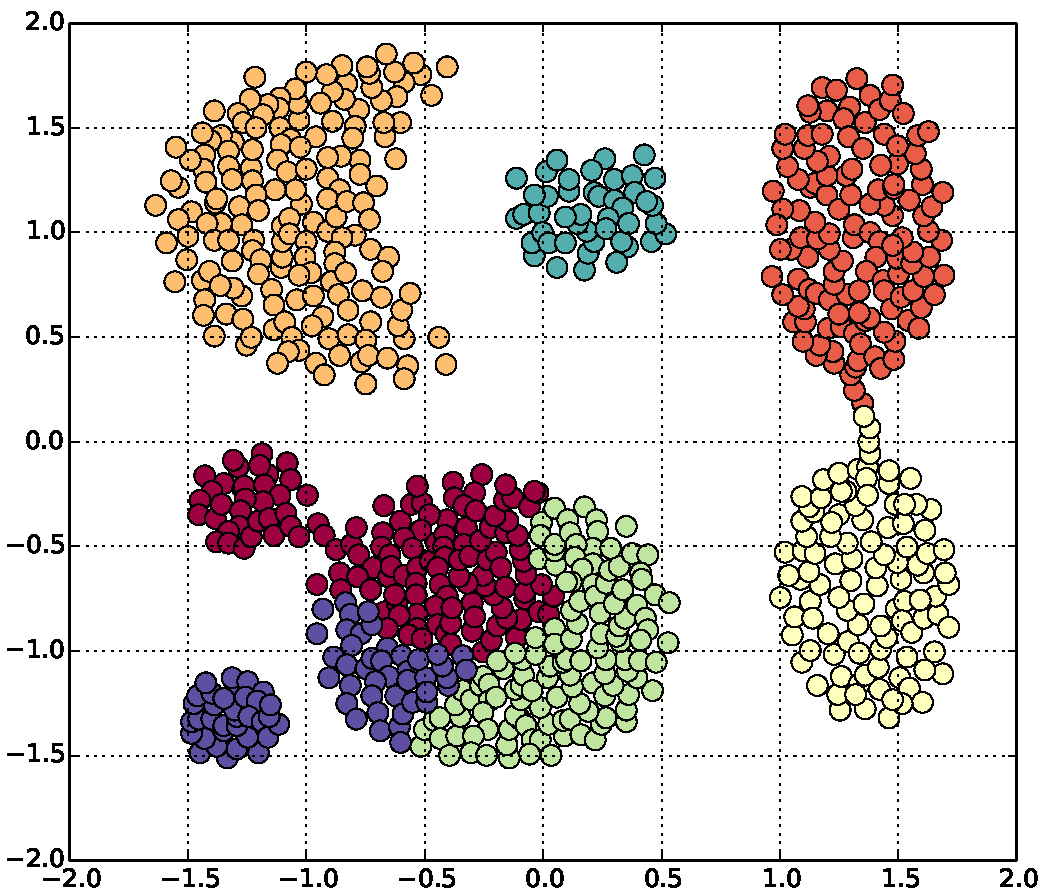
\includegraphics[height = 5cm, width = 5cm]{ward.pdf}
      \label{fig:ward}
   }
   \subfigure[DBSCAN]{
      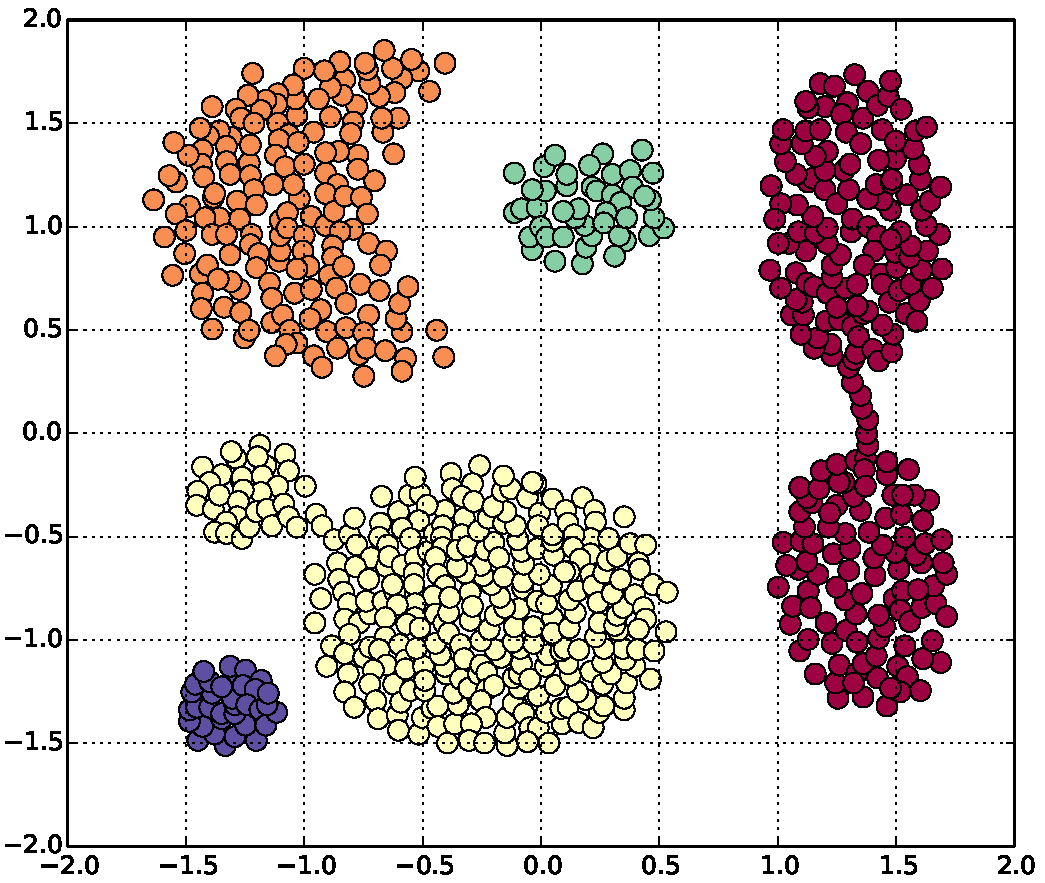
\includegraphics[height = 5cm,width = 5cm]{dbscan.pdf}
      \label{fig:dbscan}
   }
   \caption{A comparison against DBSCAN}
   \label{fig:compare}
\end{figure}

The algorithm exhibits variation in perforamce as per the standard bias-variance dilemma.
Figure~\ref{fig:error} shows how the error varies for DBSCAN when applied to data used in Figure~\ref{fig:compare}.
The EPS paramter sets the distance which the algorithm allow itself to jump and consider itself in the same cluster.

\begin{figure}[ht]
   \centering
    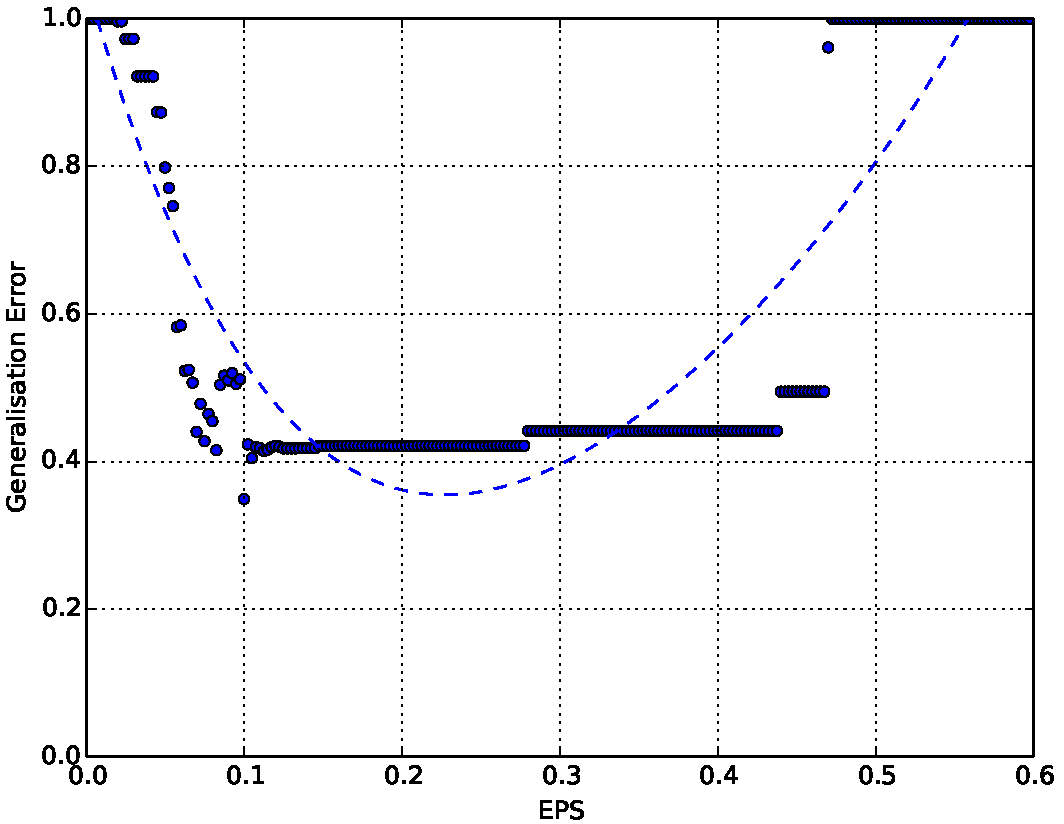
\includegraphics[height = 5cm,width = 8cm]{error.pdf}
   \caption{Generalisation error with varying input parameter}
   \label{fig:error}
\end{figure}




\section{Conclusion and Further Work}

\bibliographystyle{ecs}
\bibliography{references}



\end{document}
%% ----------------------------------------------------------------

